% siminos/talks/WoodsHole12/WHole14.tex      pdflatex sectSlice
% $Author: predrag $
% $Date: 2014-08-05 21:53:47 -0400 (Tue, 05 Aug 2014) $

% remember to always update
%	ChaosBook.org/overheads/continuous/WHole14.pdf

% Predrag GFD Woods Hole talk               2014-08-04
% abstract in predrag/lectures/GFD14/
% derived from
% Predrag GFD Woods Hole talk               2012-08-08
% Predrag GT math colloquium                2012.03.26
% talks/predrag/continuous/continuous.tex   2011.09.09
% Predrag beamer format                     2011.06.17
% Predrag                                   2011.04.12
% derived from
% siminos/talks/Dresden10/symmReduc.tex 	2010.06.29
% Predrag Eckmann's haeberli slide style    2005.05.03
%    ChaosBook/version 11 slides
%	 from ChaosBook continuous.tex

% might want to use text from
%    predrag/lectures/Goth11/Cphg11abstr.txt
%    predrag/lectures/maribor/11/abscvitancourse.tex

\input ../../inputs/layoutBeamer
\input ../../inputs/def % no edits, always from dasbuch/book/inputs
\input ../../inputs/defsBeamer
                          \date{\scriptsize\textcolor{yellow}{
% 16 March 2012
% 8 Aug 2012
4 Aug 2014
}

\bigskip

[for ChaosBook.org version click
\HREF{http://www.ChaosBook.org/}
{\textcolor{blue}{here}}]                          }

\title{{\Huge geometry of turbulence}
       \\
       (or,
       how to slice baroclinic instability)}
%\author{Predrag Cvitanovi\'c}
\author[Cvitanovi\'c]
{
  \textcolor{green!50!black}{
  {Predrag~Cvitanovi\'c}
  }
}
\institute
{
%  \inst{1}%
% CDSNS Colloquium \\
School of Physics, Georgia Tech
}

\begin{document}

\begin{frame}
  \titlepage
\end{frame}

%\begin{frame}{Outline}
%  \tableofcontents
%\end{frame}

% insert hopf04insert2.pdf

\begin{frame}{the challenge}

\bigskip

\begin{center}{\Large turbulence.zip}
\end{center}

\bigskip

    \begin{block}{or `equation assisted' data compression:}
replace the $\infty$ of
turbulent videos by the best possible
\begin{center}{\Large \textcolor{blue}{small finite set}}
\end{center}
of \textcolor{blue}{videos} encoding all physically distinct  motions of
the turbulent fluid
    \end{block}
\end{frame}

% insert hopf04insert1a.pdf

\section[baroclinic instability]{baroclinic instability}

\begin{frame}{`harmonic oscillator' of geophysical fluid dynamics}
\begin{block}{baroclinic instability}
 fundamental GFD concept: drives
large scale circulations in the atmosphere and in
the ocean
\end{block}

\bigskip

\begin{block}{baroclinity / baroclinicity}
how
misaligned is the gradient of pressure from the gradient of density in a
 stratified fluid?
\bigskip

a measure: baroclinic vector
\[
\frac{1}{\rho^2} \nabla \rho \times \nabla p
\] %ee{baroclVec}
angle between surfaces of
constant pressure (isobars) and surfaces of constant density
(isopycnic surfaces) is a source of vorticity
\end{block}

\end{frame}

\begin{frame}{geostrophic equilibria}
\begin{block}{in presence of rotation}
there are equilibrium states with isopycnals and isobars not parallel
\end{block}

\begin{block}{baroclinic instability}
occurs when the isopycnal slope exceeds a critical value
\end{block}
\end{frame}

\begin{frame}{2-layer quasigeostrophic model}
\begin{block}{}
\begin{center}
    \includegraphics[width=0.5\textwidth, clip=true]{twolayermodel}
\end{center}
\end{block}

\begin{block}{Phillips 1954; Pedlosky}
\begin{itemize}
  \item
$j$th layer vorticity
$\nabla^2 \psi_j$ given by stream function $\psi_j$
  \item  each layer is computed in terms of vorticity equations as a 2D
incompressible viscous fluid in a channel with no-slip side walls,
periodic in streamwise direction
\end{itemize}

\end{block}
\end{frame}

\begin{frame}{2-layer quasigeostrophic equations}

			\begin{exampleblock}{}
\begin{itemize}
  \item
top layer driven by constant velocity `atmospheric stream'
  \item
bottom layer no slip, no
\HREF{http://en.wikipedia.org/wiki/Ekman_layer}{Ekman layer} modeling
friction at the bottom
  \item
lower layer has higher fluid density
  \item
layers are coupled across their interface by difference of vorticity,
through $\psi_2-\psi_1$, with strength


$F \approx~(${\scriptsize Rossby deformation radius}$)^{-2}$
\end{itemize}
			\end{exampleblock}


\begin{block}{Phillips 1954}
    {\scriptsize
\begin{eqnarray}
\frac{\partial}{\partial t} \left(\nabla^2 \psi_1
+ F(\psi_2-\psi_1)\right)+\textbf{u} \cdot \nabla \left(\nabla^2 \psi_1 + F(\psi_2-\psi_1)\right)+\beta \frac{\partial \psi_1}{\partial x}
  = -\nu \nabla^2 \psi_1 \nonumber \\
\frac{\partial}{\partial t} \left(\nabla^2 \psi_2
+ F(\psi_1-\psi_2)\right)+\textbf{u} \cdot \nabla \left(\nabla^2 \psi_2 + F(\psi_1-\psi_2)\right)+\beta \frac{\partial \psi_2}{\partial x}
=-\nu \nabla^2 \psi_2
\nnu
\end{eqnarray}
    }
\end{block}
\end{frame}

\begin{frame}{domain size}

\begin{block}{computational cell}
vertical  shear characterized by $U_o$,
\begin{center}
  \includegraphics[width=0.4\textwidth]{DomainDefinition}\\
\end{center}
$x$ streamwise, $y$ spanwise
\end{block}

\begin{block}{geophysically relevant}
when zonal (streamwise) length
substantially greater than the meridional (spanwise) breadth
\end{block}
\end{frame}

\begin{frame}{numerical simulations}
\HREF{http://www.bobdylan.com/songs/subterranean-homesick-blues}
{Annalisa Bracco}
\begin{block}{}
%%%%%%%%%%%%%%%%%%%%%%%%%%%%%%%%%%%%%%%%%%%%%%%%%%%%%%%%%%%%%%%%%%%%%
\begin{center}
    \includegraphics[width=0.55\textwidth]{111028layer1}
\end{center}
A plot of the vorticity in the top layer at 4 different times
%\label{f:111028layer1}
%%%%%%%%%%%%%%%%%%%%%%%%%%%%%%%%%%%%%%%%%%%%%%%%%%%%%%%%%%%%%%%%%%%%%
\end{block}
\end{frame}

\begin{frame}{baroclinic flow}
\begin{block}{}
%%%%%%%%%%%%%%%%%%%%%%%%%%%%%%%%%%%%%%%%%%%%%%%%%%%%%%%%%%%%%%%%%%%%%
\begin{center}
\HREF{../../movies/BaroclinicSlice4.avi}
{\textcolor{red}{click here - a simulation}}
\end{center}
A DNS of the vorticity in the top layer
%\label{f:111028layer1}
%%%%%%%%%%%%%%%%%%%%%%%%%%%%%%%%%%%%%%%%%%%%%%%%%%%%%%%%%%%%%%%%%%%%%
\end{block}

\vfill

{\scriptsize Sebastian Ortega Arango, code by
\HREF{http://www.bobdylan.com/songs/subterranean-homesick-blues}
{Annalisa Bracco}
}
\end{frame}


\section[dynamical systems]{dynamical systems}

\begin{frame}{\statesp}
construct \statesp\ orthogonal basis sets using the Euclidean inner
product

\bigskip
numerical fluids:  PDE discretization independent L2 norm is
\begin{block}{energy norm}
\[
  \Norm{\bu-\bv}^2  = \braket{\bu-\bv}{\bu-\bv}  = \frac{1}{V}
                \int_\bCell \! d \bx \;
                       (\bu-\bv) \cdot (\bu-\bv)
%\label{innerproduct}
\]
\end{block}
\end{frame}

\renewcommand{\ssp}{\ensuremath{a}}                % state space point

\begin{frame}{orthonormal basis set}
construct
\[
\{\be_1, \be_2, \cdots, \be_n\}, \qquad \Norm{\be_j}=1
\]

by picking instantaneous snapshots
\(
\bu = \bu(x,y,\zeit)
\)
of steady turbulence states at arbitrary
times $\zeit$, orthogonalize

\bigskip

example : spanwise reflection is a symmetry, so can construct
an orthonormal pair of basis vectors
\[ %beq
\be_{1,2} = \frac{\bu(x,y) \pm \bu(x,-y)}{\Norm{\bu(x,y) \pm \bu(x,-y)}}
\,.
\] %ee{antisymBasis}
\end{frame}

\begin{frame}{basis set $\{\be_1, \be_2, \cdots, \be_n\}$}
\begin{block}{}
%%%%%%%%%%%%%%%%%%%%%%%%%%%%%%%%%%%%%%%%%%%%%%%%%%%%%%%%%%%%%%%%%%%%%
\begin{center}
    \includegraphics[width=0.75\textwidth]{Projectionvectors}
\end{center}
%%%%%%%%%%%%%%%%%%%%%%%%%%%%%%%%%%%%%%%%%%%%%%%%%%%%%%%%%%%%%%%%%%%%%
\end{block}
orthonormal, as $\be_1$ basis vector corresponds to an antisymmetric fluid state,
and $\be_2$ to a symmetric one, \etc
\end{frame}

\begin{frame}{projections onto basis vectors $(\ssp_1, \ssp_2)$}
\begin{block}{}
\[
\ssp_j(\zeit)  = \braket{\be_{j}}{u(\zeit)}
=\Re \left[\sum_{n=1}^2\sum_{l=0}^{M-1}\sum_{k=0}^{N/2}
u_{lkn}(\zeit) e^i_{lkn} \right]
\,,
\] % ee{dotProduct}
$j$ labels the basis vector
\\
$n$ labels the layers,
\\
computational basis:
$k$ for the streamwise Fourier mode, \etc
\end{block}
\end{frame}

\begin{frame}{can visualize 61,506 dimensional \statesp\ of turbulent flow}
\begin{center}
\includegraphics[width=0.80\textwidth]{statespace_123}
\end{center}
\eqva\ of turbulent plane Couette flow,
\\
their unstable manifolds, and
\\
myriad of turbulent videos mapped out as one happy family

\bigskip

\hfill   \vfill

{\scriptsize
          for movies, please click through
            \textcolor{blue}{\href{http://ChaosBook.org/tutorials}
             {ChaosBook.org/tutorials}}
          }
\end{frame}

\renewcommand{\ssp}{\ensuremath{x}}                % state space point

%%%%%%%%%%%%%%%%%%%%%%%%%%%%%%%%%%%%%%%%%%%%%%%%%%%%%%%%%%%%%%%%%%%%%%%%%%%%
\section[Das Problem]{the problem with symmetry}

\begin{frame}{however, if there are symmetries...}
\begin{block}{a coordinate transformation $\LieEl$
\\
is a {symmetry} of the dynamics if}
for every solution $\flow{\zeit}{\ssp}$

\medskip

$\LieEl \flow{\zeit}{\ssp} = \flow{\zeit}{\LieEl\ssp}$ is also a solution
\end{block}

\bigskip

\begin{block}{a flow $\dot{\ssp}= \vel(\ssp)$ is $\Group$-equivariant if}
equations of motion have the same form in all frames
\[
\vel(\ssp)=\LieEl^{-1} \, \vel(\LieEl \, \ssp)
\,,\qquad \mbox{for all } \LieEl \in {\Group}
\,.
\] %ee{eq:FiniteRot}
\end{block}

\end{frame}


\begin{frame}{example : symmetries of pipe flow}
            \begin{block}{}
 %% A27*-pipeSymms.* - read dasbuch/book/FigSrc/inkscape/00ReadMe.txt
 \begin{center}
  \setlength{\unitlength}{0.35\textwidth}
  %% \unitlength = units used in the Picture Environment
(a)
  \begin{picture}(1,0.52454249)%
    \put(0,0){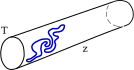
\includegraphics[width=\unitlength]{A27a-pipeSymms}}%
    \put(0.61583231,0.13683004){\color[rgb]{0,0,0}\makebox(0,0)[lb]{\smash{$z$}}}%
    \put(0.00611823,0.27217453){\color[rgb]{0,0,0}\makebox(0,0)[lb]{\smash{$\theta$}}}%
  \end{picture}%
(b)
  \begin{picture}(1,0.52454249)%
    \put(0,0){\includegraphics[width=\unitlength]{A27b-pipeSymms}}%
    \put(0.61583231,0.13683004){\color[rgb]{0,0,0}\makebox(0,0)[lb]{\smash{$z$}}}%
    \put(0.00611823,0.27217453){\color[rgb]{0,0,0}\makebox(0,0)[lb]{\smash{$\theta$}}}%
  \end{picture}%
\\
(c)
  \begin{picture}(1,0.52454249)%
    \put(0,0){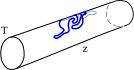
\includegraphics[width=\unitlength]{A27c-pipeSymms}}%
    \put(0.61583231,0.13683004){\color[rgb]{0,0,0}\makebox(0,0)[lb]{\smash{$z$}}}%
    \put(0.00611823,0.27217453){\color[rgb]{0,0,0}\makebox(0,0)[lb]{\smash{$\theta$}}}%
  \end{picture}%
(d)
  \begin{picture}(1,0.52454249)%
    \put(0,0){\includegraphics[width=\unitlength]{A27d-pipeSymms}}%
    \put(0.61583231,0.13683004){\color[rgb]{0,0,0}\makebox(0,0)[lb]{\smash{$z$}}}%
    \put(0.00611823,0.27217453){\color[rgb]{0,0,0}\makebox(0,0)[lb]{\smash{$\theta$}}}%
  \end{picture}%
 \end{center}
a fluid state shifted by a stream-wise translation and azimuthal rotation
is a physically equivalent state
			\end{block}
%	\end{columns}
% \caption{\label{fig:A27-pipeSymms}
			\begin{exampleblock}{}
\begin{itemize}
  \item[b)]  stream-wise
  \item[c)]  stream-wise, azimuthal
  \item[d)]  azimuthal flip
\end{itemize}
			\end{exampleblock}
\end{frame}

\begin{frame}{trajectories, orbits}
%  \caption{\label{fig:A27wurst} from atlas12
  \setlength{\unitlength}{0.28\textwidth}
\begin{center}
{\scriptsize %small
(a)
  \begin{picture}(1,0.98239821)%
    \put(0,0){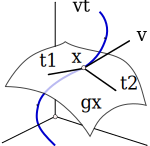
\includegraphics[width=\unitlength]{A28tangent3}}%
    \put(0.91612064,0.70682767){\color[rgb]{0,0,0}\makebox(0,0)[lb]{\smash{$\vel$}}}%
    \put(0.48698745,0.90266503){\color[rgb]{0,0,0}\makebox(0,0)[lb]{\smash{$\ssp(\zeit)$}}}%
    \put(0.2624318,0.5347756){\color[rgb]{0,0,0}\makebox(0,0)[lb]{\smash{$\groupTan_1$}}}%
    \put(0.80471037,0.38188675){\color[rgb]{0,0,0}\makebox(0,0)[lb]{\smash{$\groupTan_2$}}}%
    \put(0.538343,0.25344355){\color[rgb]{0,0,0}\makebox(0,0)[lb]{\smash{$\pS_\ssp$}}}%
    \put(0.47864531,0.56060893){\color[rgb]{0,0,0}\makebox(0,0)[lb]{\smash{$\ssp$}}}%
  \end{picture}%
~~~~~~~(b)
  \begin{picture}(1,0.9071451)%
    \put(0,0){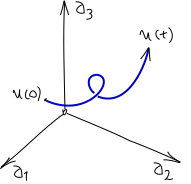
\includegraphics[width=\unitlength]{A27traj}}%
    \put(0.81413243,0.74633551){\color[rgb]{0,0,0}\makebox(0,0)[lb]{\smash{$\ssp(\zeit)$}}}%
    \put(0.14085867,0.30233715){\color[rgb]{0,0,0}\makebox(0,0)[lb]{\smash{$\ssp(0)$}}}%
  \end{picture}%
\\
(c)
	\begin{picture}(1,0.88265338)%
    \put(0,0){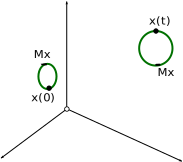
\includegraphics[width=\unitlength]{A27gOrbit}}%
    \put(0.17017404,0.30123416){\color[rgb]{0,0,0}\makebox(0,0)[lb]{\smash{$\ssp(0)$}}}%
    \put(0.10473094,0.59736144){\color[rgb]{0,0,0}\makebox(0,0)[lb]{\smash{$\pS_{\ssp(0)}$}}}%
    \put(0.80073137,0.42842331){\color[rgb]{0,0,0}\makebox(0,0)[lb]{\smash{$\pS_{\ssp(\zeit)}$}}}%
    \put(0.81421682,0.75061198){\color[rgb]{0,0,0}\makebox(0,0)[lb]{\smash{$\ssp(\zeit)$}}}%
	\end{picture}%
~~~~~~~(d)
	\begin{picture}(1,0.90708568)%
    \put(0,0){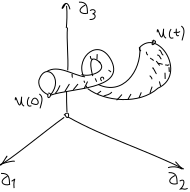
\includegraphics[width=\unitlength]{A27wurst}}%
    \put(0.81871555,0.75240026){\color[rgb]{0,0,0}\makebox(0,0)[lb]{\smash{$\ssp(\zeit)$}}}%
    \put(0.12337724,0.29209515){\color[rgb]{0,0,0}\makebox(0,0)[lb]{\smash{$\ssp(0)$}}}%
	\end{picture}%
} %end {\small
\end{center}

	\begin{columns}[t]
	\column{.65\textwidth}
(a) $\ssp$ tangent vectors:

\medskip

$\vel(\ssp)$ along time flow $\ssp(\zeit)$
\\
$\groupTan_1(\ssp),\, \cdots, \groupTan_N(\ssp)$
group tangents
	\column{.35\textwidth}
%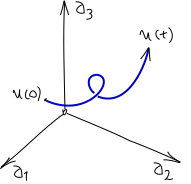
\includegraphics[width=0.95\textwidth]{A27traj}
(b) trajectory $\ssp(\zeit)$
%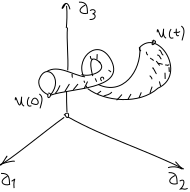
\includegraphics[width=0.95\textwidth]{A27wurst}

\medskip

%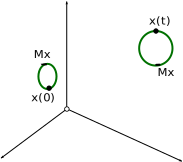
\includegraphics[width=0.95\textwidth]{A27gOrbit}
(c) group orbits $\LieEl\,\ssp(\zeit)$

\medskip

(d) wurst $\LieEl\,\ssp(\zeit)$
	\end{columns}
\end{frame}

\section[relativity for cyclists]{relativity for cyclists}

\subsection[in/equivariance]{}

\begin{frame}{foliation by group orbits}
  \begin{columns}
  \column{0.5\textwidth}
\begin{block}{group orbits}
% 2011-08-23 Predrag: previously BeThTraj.pdf from
% dasbuch/book/FigSrc/inkscape/BeThTraj.svg
%  2011-09-09 Predrag: updated continuous.tex overheads
%  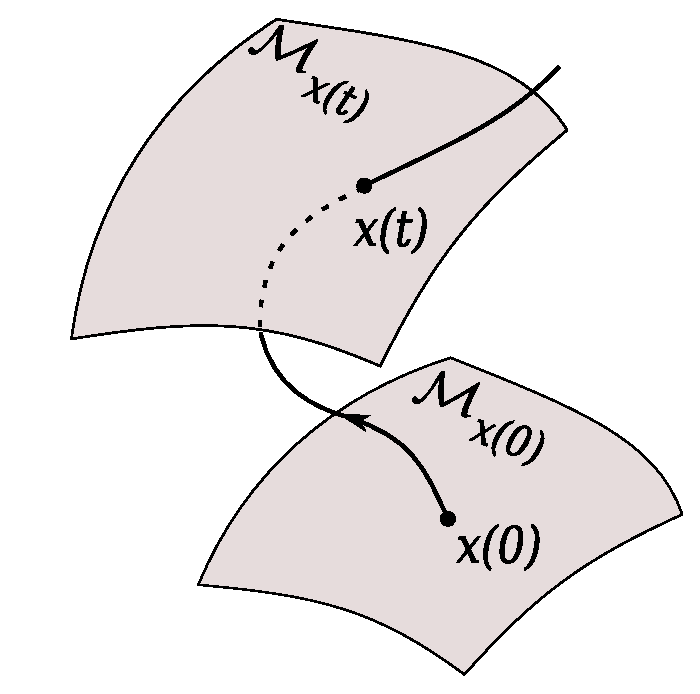
\includegraphics[width=1.00\textwidth,clip=true]{BeThTraj}
 \begin{center}
  \setlength{\unitlength}{1.00\textwidth}
  %% \unitlength = units used in the Picture Environment
  {\small
\only<1-2>{
  \begin{picture}(1,0.98655417)%
    \put(0,0){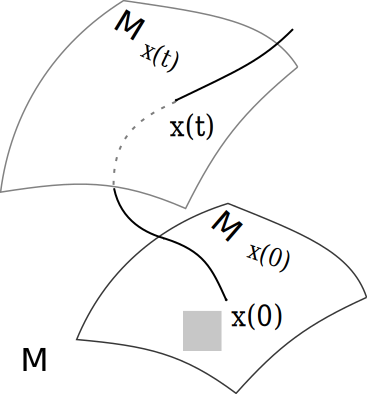
\includegraphics[width=\unitlength]{BeThTrajTeX}}%
    \put(0.35976094,0.91875614){\color[rgb]{0,0,0}\rotatebox{-16.32889204}{\makebox(0,0)[lb]{\smash{$\pS_{\ssp(\zeit)}$}}}}%
        \put(0.60333631,0.42274457){\color[rgb]{0,0,0}\rotatebox{-30.8073288}{\makebox(0,0)[lb]{\smash{$\pS_{\ssp(0)}$}}}}%
    \put(0.63001383,0.14959019){\color[rgb]{0,0,0}\rotatebox{0.0313674}{\makebox(0,0)[lb]{\smash{$\ssp(0)$}}}}%
    \put(0.4558276,0.64524238){\color[rgb]{0,0,0}\rotatebox{0.0313674}{\makebox(0,0)[lb]{\smash{$\ssp(\zeit)$}}}}%
    \put(0.13110825,0.05766516){\color[rgb]{0,0,0}\rotatebox{0.11031334}{\makebox(0,0)[lb]{\smash{$\pS$}}}}%
  \end{picture}%
  }
\only<3>{
  \begin{picture}(1,0.97809647)%
    \put(0,0){\includegraphics[width=\unitlength]{BeThFoliTeX}}%
    \put(0.35673326,0.91086901){\color[rgb]{0,0,0}\rotatebox{-31.32889204}{\makebox(0,0)[lb]{\smash{$\pS_{\ssp(\zeit)}$}}}}%
    \put(0.8041738,0.27513933){\color[rgb]{0,0,0}\rotatebox{-40.8073288}{\makebox(0,0)[lb]{\smash{$\pS_{\ssp(0)}$}}}}%
    \put(0.64701656,0.09606165){\color[rgb]{0,0,0}\rotatebox{0.0313674}{\makebox(0,0)[lb]{\smash{$\ssp(0)$}}}}%
    \put(0.50157066,0.63965709){\color[rgb]{0,0,0}\rotatebox{0.0313674}{\makebox(0,0)[lb]{\smash{$\ssp(\zeit)$}}}}%
    \put(0.13000487,0.05702481){\color[rgb]{0,0,0}\rotatebox{0.11031334}{\makebox(0,0)[lb]{\smash{$\pS$}}}}%
  \end{picture}%
  }
  } % end {\small %scriptsize
 \end{center}
\end{block}
  \column{0.5\textwidth}
		\only<1>{
\noindent
\emph{group orbit} $\pS_\ssp $ of $\ssp$ is the set of all group
actions
\[
\pS_\ssp = \{\LieEl\,\ssp \mid \LieEl \in {\Group}\}
\]
        }
		\only<2>{
%\noindent
%group orbit $\pS_{\ssp(0)}$ of \statesp\ point
% $\ssp(0)$, and the group orbit $\pS_{\ssp(\zeit)}$
%reached by the trajectory $\ssp(\zeit)$ time $t$ later.
%        }
%		\only<3>{
\noindent
any point on the manifold $\pS_{\ssp(\zeit)}$ is
equivalent to any other
        }
		\only<3>{
\noindent
action of a symmetry group
foliates the \statesp\ $\pS$ into a union of group
orbits $\pS_{\ssp}$

\medskip

each group orbit $\pS_{\ssp}$ is an equivalence class
        }
\end{columns}
\end{frame}

\section{symmetry reduction}

\begin{frame}{}
\begin{block}{the goal}
replace each group orbit by a unique
point in a lower-dimensional

\bigskip

\hfill
\textcolor{red}{\Large symmetry \reducedsp\ $\pS/\Group$}
\end{block}
\end{frame}

\begin{frame}{symmetry reduction}
  \begin{columns}
  \column{0.5\textwidth}
\begin{block}{full \statesp}
 \begin{center}
  \setlength{\unitlength}{1.00\textwidth}
  %% \unitlength = units used in the Picture Environment
  \begin{picture}(1,0.98655417)%
    \put(0,0){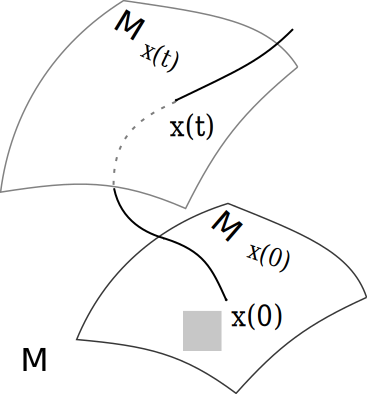
\includegraphics[width=\unitlength]{BeThTrajTeX}}%
    \put(0.35976094,0.91875614){\color[rgb]{0,0,0}\rotatebox{-16.32889204}{\makebox(0,0)[lb]{\smash{$\pS_{\ssp(\zeit)}$}}}}%
        \put(0.60333631,0.42274457){\color[rgb]{0,0,0}\rotatebox{-30.8073288}{\makebox(0,0)[lb]{\smash{$\pS_{\ssp(0)}$}}}}%
    \put(0.63001383,0.14959019){\color[rgb]{0,0,0}\rotatebox{0.0313674}{\makebox(0,0)[lb]{\smash{$\ssp(0)$}}}}%
    \put(0.4558276,0.64524238){\color[rgb]{0,0,0}\rotatebox{0.0313674}{\makebox(0,0)[lb]{\smash{$\ssp(\zeit)$}}}}%
    \put(0.13110825,0.05766516){\color[rgb]{0,0,0}\rotatebox{0.11031334}{\makebox(0,0)[lb]{\smash{$\pS$}}}}%
  \end{picture}%
 \end{center}
\end{block}
  \column{0.5\textwidth}
\begin{block}{\reducedsp}
 \begin{center}
  \setlength{\unitlength}{1.00\textwidth}
  %% \unitlength = units used in the Picture Environment
  \begin{picture}(1,1.07315413)%
    \put(0,0){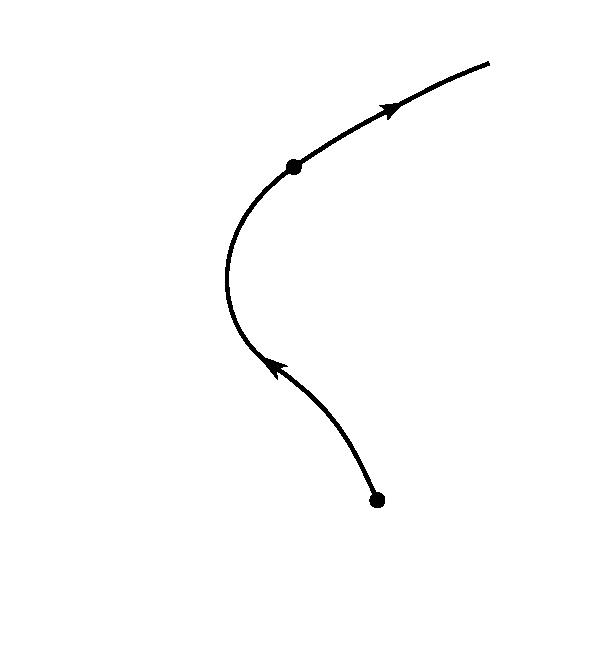
\includegraphics[width=\unitlength]{BeThRedTeX}}%
    \put(0.19912369,0.17144733){\color[rgb]{0,0,0}\rotatebox{0.11031334}{\makebox(0,0)[lb]{\smash{$\pSRed$}}}}%
    \put(0.63028127,0.18433598){\color[rgb]{0,0,0}\rotatebox{0.03136739}{\makebox(0,0)[lb]{\smash{$\sspRed(0)$}}}}%
    \put(0.46253394,0.70182305){\color[rgb]{0,0,0}\rotatebox{0.03136739}{\makebox(0,0)[lb]{\smash{$\sspRed(\tau)$}}}}%
  \end{picture}%
 \end{center}
\end{block}
\end{columns}
\end{frame}

\begin{frame}{relativity for cyclists}
\begin{block}{\mslices}

\bigskip
cut group orbits by a hypersurface
\textcolor{red}{(not a Poincar\'e section)}, each group orbit of
symmetry-equivalent points represented by the single point
\end{block}
%\bigskip
%\textcolor{blue}{\Large cut how?}
\end{frame}

\section{slice \& dice}


\begin{frame}{chosing a `slice' hyperplane}
  \begin{columns}
  \column{0.50\textwidth}
%\begin{block}{}
flow field at the \statesp\
point $\ssp$ induced by the action of the group is given by
the set of $N$ \emph{tangent fields}
\[
\groupTan_a(\ssp)_{i}= (\Lg_a){}_{ij} \ssp_j
\] %{GroupTangField}
%\end{block}
  \column{0.40\textwidth}
\begin{block}{group tangent fields} %group orbits}
 \begin{center}
  \setlength{\unitlength}{0.80\textwidth}
{\scriptsize %small
  \begin{picture}(1,0.98239821)%
    \put(0,0){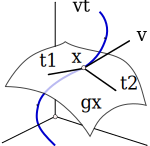
\includegraphics[width=\unitlength]{A28tangent3}}%
    \put(0.91612064,0.70682767){\color[rgb]{0,0,0}\makebox(0,0)[lb]{\smash{$\vel$}}}%
    \put(0.48698745,0.90266503){\color[rgb]{0,0,0}\makebox(0,0)[lb]{\smash{$\ssp(\zeit)$}}}%
    \put(0.2624318,0.5347756){\color[rgb]{0,0,0}\makebox(0,0)[lb]{\smash{$\groupTan_1$}}}%
    \put(0.80471037,0.38188675){\color[rgb]{0,0,0}\makebox(0,0)[lb]{\smash{$\groupTan_2$}}}%
    \put(0.538343,0.25344355){\color[rgb]{0,0,0}\makebox(0,0)[lb]{\smash{$\pS_\ssp$}}}%
    \put(0.47864531,0.56060893){\color[rgb]{0,0,0}\makebox(0,0)[lb]{\smash{$\ssp$}}}%
  \end{picture}%
}
 \end{center}
\end{block}
  \end{columns}
% \bigskip

\begin{block}{infinitesimal transformations}
\[
\LieEl
 \simeq  1 + \gSpace \cdot \Lg \,, \qquad \vert \delta \gSpace \vert \ll 1
\]
\end{block}

\begin{block}{slice condition}
\[ %beq
 \braket{\sspRed}{\sliceTan{a}}
   = 0
    \,,\qquad
	  \sliceTan{a} = \Lg_a \slicep
\] % ee{PCsectQ0}
\end{block}
\end{frame}

\begin{frame}{flow within the slice}
\slice\ hyperplane : normal to group tangent $\sliceTan{}$ at template  $\slicep{}$

\bigskip
	\begin{exampleblock}
          {\reducedsp\ $\pSRed$  flow $\velRed(\sspRed)$}
\bea
\velRed(\sspRed) &=& \vel(\sspRed)
                    \,-\, \dot{\gSpace}(\sspRed)  \cdot \groupTan(\sspRed)
    \,,\qquad\quad \sspRed \in \pSRed
\continue
\dot{\gSpace}_a(\sspRed) &=& \braket{\vel(\sspRed)^T}{\sliceTan{a}}
                       /\braket{\groupTan(\sspRed)^T}{\sliceTan{}}
\,.
\nnu %\label{EqMotMFrame}
\eea
	\end{exampleblock}
\begin{itemize}
  \item $\vel$ : velocity, full space
  \item $\velRed$ : velocity component in slice
  \item $\dot{\gSpace}  \cdot \groupTan$ : velocity component normal to slice
  \item $\dot{\gSpace}$ : reconstruction equation for the group phases
\end{itemize}
\end{frame}

\begin{frame}{flow within the slice}
\begin{block}{} %group orbits}
\begin{center}
  \setlength{\unitlength}{0.70\textwidth}
  \begin{picture}(1,0.87085079)%
    \put(0,0){\includegraphics[width=\unitlength]{slice}}%
    \put(0.82835155,0.19007659){\color[rgb]{0,0,0}\rotatebox{-14.84025424}{\makebox(0,0)[lb]{\smash{$\pSRed$}}}}%
    \put(0.06577338,0.24688228){\color[rgb]{0,0,0}\rotatebox{0.0313674}{\makebox(0,0)[lb]{\smash{$\LieEl\,\slicep$}}}}%
    \put(0.53023327,0.21593335){\color[rgb]{0,0,0}\rotatebox{0.0313674}{\makebox(0,0)[lb]{\smash{$\slicep$}}}}%
    \put(0.3184954,0.089285){\color[rgb]{0,0,0}\rotatebox{0.0313674}{\makebox(0,0)[lb]{\smash{$\sliceTan{}$}}}}%
    \put(0.00008985,0.35305068){\color[rgb]{0,0,0}\rotatebox{0.0313674}{\makebox(0,0)[lb]{\smash{$\ssp(\zeit)$}}}}%
    \put(0.69766235,0.41412105){\color[rgb]{0,0,0}\rotatebox{0.0313674}{\makebox(0,0)[lb]{\smash{$\sspRed(\zeit)$}}}}%
    \put(0.06716446,0.70280851){\color[rgb]{0,0,0}\rotatebox{0.0313674}{\makebox(0,0)[lb]{\smash{$\LieEl\,\ssp(\zeit)$}}}}%
  \end{picture}%
%  \includegraphics[width=0.70\textwidth,clip=true]{sliceRaw}
\end{center}
\end{block}
full-space trajectory $\ssp(\tau)$ \\
rotated into the \reducedsp\ $\sspRed(\tau) = \LieEl(\gSpace)^{-1}\ssp(\tau)$ \\
by appropriate \emph{moving frame} angles $\{\gSpace(\tau)\}$
\end{frame}

\begin{frame}{symmetry reduced baroclinic flow}
\begin{block}{}
%%%%%%%%%%%%%%%%%%%%%%%%%%%%%%%%%%%%%%%%%%%%%%%%%%%%%%%%%%%%%%%%%%%%%
\begin{center}
\HREF{../../movies/BaroclinicSlice.avi}
{\textcolor{red}{click here - a simulation}}
\end{center}
A DNS of the vorticity in the top layer
%\label{f:111028layer1}
%%%%%%%%%%%%%%%%%%%%%%%%%%%%%%%%%%%%%%%%%%%%%%%%%%%%%%%%%%%%%%%%%%%%%
\end{block}

\vfill

{\scriptsize Sebastian Ortega Arango}
\end{frame}

\begin{frame}{\rpo}
a \rpo\ $p$ is an orbit in
{\statesp} $\pS$ which exactly recurs
%    \PC{create SFIG here}
\beq
\ssp_p (\zeit) = g_p \ssp_p (\zeit + \period{p} )
    \,,\qquad
\ssp_p (\zeit) \in \pS_p
\label{RPOrelper1}
\eeq
for a fixed \textcolor{blue}{relative period} $\period{p}$
and a fixed group action ${g_p} \in  \Group$
that shifts the endpoint $\ssp_p (\period{p} ) $
back into the initial point $\ssp_p (0) $.
\end{frame}


\begin{frame}{\rpo $\to$ \po}
%%%%%%%%%%%%%%%%%%%%%%%%%%%%%%%%%%%%%%%%%%%%%%%%%%%%%%%%%%%%%%%%
%% slice.*, inflectHype.*: see dasbuch/book/FigSrc/inkscape/00ReadMe.txt
%% rpo.* hand-drawn in dasbuch/book/FigSrc/xfig/rpo.fig
%% xfig exported -> FigSrc/inkscape/rpo.fig
%% inkscape exported -> rpo.eps + LaTeX, hand edited in the macros
%% Predrag 2011-08-27 replaced rpo.pdf by rpoSlice.pdf
%%  2011-09-09 Predrag: updated continuous.tex overheads
%% remember to insert rpoSlice.pdf into ChaosBook
\begin{block}{}
 \begin{center}
  \setlength{\unitlength}{0.70\textwidth}
  %% \unitlength = units used in the Picture Environment
  \begin{picture}(1,0.87085079)%
    \put(0,0){\includegraphics[width=\unitlength]{rpoSlice}}%
    \put(0.82835153,0.19007656){\color[rgb]{0,0,0}\rotatebox{-14.84025432}{\makebox(0,0)[lb]{$\pSRed$}}}%
    \put(0.38925459,0.38713857){\color[rgb]{0,0,0}\rotatebox{0.0313674}{\makebox(0,0)[lb]{\smash{$\ssp(0)$}}}}%
    \put(0.70354118,0.30765314){\color[rgb]{0,0,0}\rotatebox{0.0313674}{\makebox(0,0)[lb]{\smash{$\sspRed(\zeit)$}}}}%
    %\put(0.40171187,0.21813817){\color[rgb]{0,0,0}\rotatebox{0.0313674}{\makebox(0,0)[lb]{\smash{$\LieEl(\zeit)$}}}}%
    \put(0.00068739,0.2359574){\color[rgb]{0,0,0}\rotatebox{0.0313674}{\makebox(0,0)[lb]{\smash{$\ssp(\zeit)$}}}}%
    \put(0.12576193,0.3969256){\color[rgb]{0,0,0}\rotatebox{0.0313674}{\makebox(0,0)[lb]{\smash{$\ssp(\period{p})$}}}}%
    \put(0.54113911,0.43476963){\color[rgb]{0,0,0}\rotatebox{0.0313674}{\makebox(0,0)[lb]{\smash{$\sspRed(0)$}}}}%
    %\put(0.06716446,0.70280851){\color[rgb]{0,0,0}\rotatebox{0.0313674}{\makebox(0,0)[lb]{\smash{$\LieEl\,\ssp(\period{})$}}}}%
  \end{picture}%
 \end{center}
\end{block}
full \statesp\ \rpo\ $\ssp(\tau)$ \\
is rotated into the \reducedsp\ {\po}
\end{frame}

\begin{frame}{}
		\only<1>{
\begin{block}{in full \statesp}
        }
		\only<2>{
\begin{block}{in \slice}
        }
\begin{center}
		\only<1>{
(\textit{a})
  \includegraphics[width=0.40\textwidth,height=0.5\textheight,clip=true]
  {ks22rpo033p50_04p045E2}
        }
		\only<2>{
(\textit{b})
  \includegraphics[width=0.40\textwidth,height=0.5\textheight,clip=true]
  {ks22rpo033p50_04p045E2CM}
        }
\end{center}
\end{block}
		\only<1>{
a \rpo\ of the Kuramoto-Sivashinsky flow, 128$d$ \statesp\
traced for four periods
 $\period{p}$, projected on

\bigskip
full \statesp\ coordinate frame
 $\{v_1,v_2,v_3\}$; a mess
        }
		\only<2>{
a \rpo\ of the Kuramoto-Sivashinsky flow projected on

\bigskip
a slice $\{\tilde{v}_1,\tilde{v}_2,\tilde{v}_3\}$ frame
        }
\end{frame}

\begin{frame}{example : pipe flow \rpo}
  \begin{columns}
  \column{0.48\textwidth}
\begin{block}{3 repeats, full space}
\includegraphics[width=1.00\textwidth,clip=true]{2841GO3a}%
\end{block}
  \column{0.48\textwidth}
\begin{block}{reduced space}
\includegraphics[width=1.00\textwidth,clip=true]{2841GO3b}%
\end{block}
  \end{columns}
\end{frame}

\begin{frame}{}
rotation into a slice \textcolor{red}{is the full snapshot}
 of the flow embedded in the

\begin{center}
\textcolor{red}{\Large $\infty$-dimensional \statesp}
\end{center}

\bigskip\bigskip
\textcolor{red}{\Large NO information} is lost by symmetry reduction
\begin{itemize}
  \item not modeling by a few degrees of freedom
  \item no dimensional reduction
\end{itemize}
\end{frame}

\section[Summary]{conclusions}


\begin{frame}{summary}
\begin{block}{symmetry reduction achieved!}
\begin{itemize}
 \item families of solutions are mapped to a single solution
    \begin{itemize}
 \item travelling waves become \eqva
 \item \rpo s become \po s
    \end{itemize}
\end{itemize}
\end{block}

\begin{block}{to be done}
\begin{itemize}
  \item construct Poincar\'e sections
  \item use the information quantitatively (periodic orbit theory)
\end{itemize}
\end{block}
\end{frame}

\begin{frame}{\Large take-home message}
if you have a symmetry
\begin{center}
\textcolor{red}{\Large use it!}
\end{center}

\bigskip\bigskip
without symmetry reduction, no understanding of fluid
flows possible
\end{frame}


% \section[flotsam]{flotsam}


\end{document}
